\documentclass[a4paper,11pt]{article}

\usepackage[T1]{polski}
\usepackage[utf8]{inputenc}
\usepackage{verbatim}
\usepackage{graphics}
\usepackage{graphicx}
\usepackage{csvsimple}
\usepackage[figurename=Zrzut\ ekranu]{caption}

\hoffset=-3.0cm                         
\textwidth=18cm                         
\evensidemargin=0pt

\voffset=-3cm                           
\textheight=27cm                        

\setlength{\parindent}{0pt}             
\setlength{\parskip}{\medskipamount}    
\raggedbottom              

\title{Postępy prac projktu indywidualnego - cz. 2}
\author{Michał Banaszczak}
\date{6 czerwca 2022} 

\begin{document}

\maketitle

\section{Napotkane problemy}

\subsection{Dynamiczna zawartość strony z danymi zawodników}
Na kolejnej stronie IO tym razem z danymi medalistów poszczególnych Igrzysk
również wykorzystano dynamiczne doładowywanie elementów w trakcie przeglądania,
zamiast załadowania wszystkiego na raz. Mianowicie jest to lista zawodników, która
przy każdym doładowaniu powiększa się o kolejnych dziesięciu atletów. Guzik do
ładowania dalszej części listy (oczywiście) jest niszczony i później tworzony nowy.
Poniżej przedstawiono działanie aplikacji.
\begin{figure}[h!t]
    \centering
    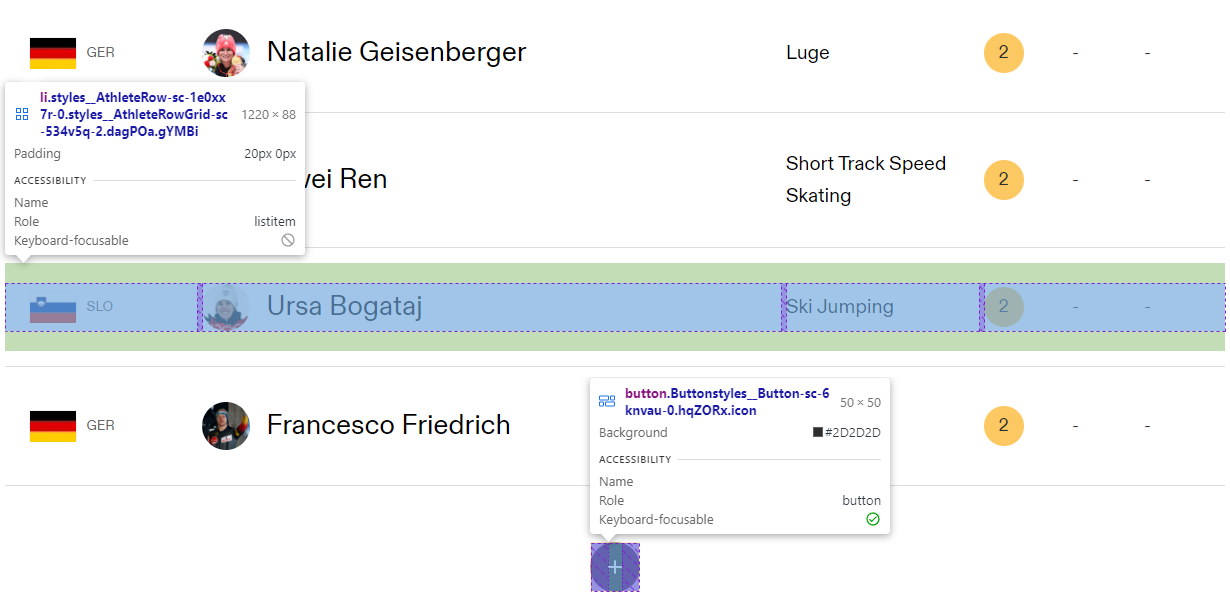
\includegraphics[width=\linewidth]{fragmentlisty.png}
    \caption{Fragment listy zawodników}
\end{figure}
\begin{figure}[h!t]
    \centering
    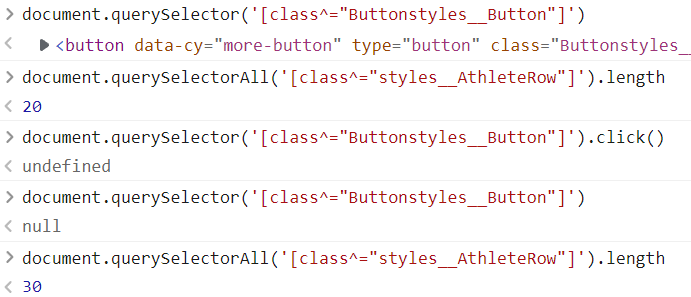
\includegraphics[width=0.65\linewidth]{zachowanielisty.png}
    \caption{Zachowanie strony przy doładowywaniu kolejnych zawodników}
\end{figure}
\newline
Ciągłe pojawianie się i znikanie guzika pozwoliło jednak na ponowne zastosowanie 
zastosowanie observera do obserwacji mutacji dokumentu, w oczekiwaniu na ponowne
pojawienie się tego guzika. Później, gdy guzik przestaje się już pokazywać po
załadowaniu całej zawartości callback wywoływany przez timeout scrapuje całą 
tabelę i rozwiązuje promise, który zwraca te dane ze skryptu ewaluacyjnego do
skryptu w Node. Moduł ten pobiera dane medalistów z tegorocznych Igrzysk zimowych
w Pekinie, natomiast łatwo można go dostosować do pobierania danych z dowolnych
Igrzysk. 

\subsection{Brak spójności nazw państw uczestniczących i przypisów}
Na poszczególnych podstronach z niewiadomych na pierwszy rzut oka zamiast nazw
państw uczestniczących figurują trzyliterowe kody. Te z kolei nie są oficjalnymi
kodami państw, a wymyślonymi specjalnie na potrzeby IO (np. \textit{SUI} dla
Szwajcarji zamiast oficjalnego \textit{CHE}). Dodatkowo w IO brały udział państwa
już nie istniejące lub różne sportowe organizacje pozapaństwowe. Z tego względu
jedynym wyjściem ujednolicenia zbioru było zmapowanie wszystkich występujących
kodów i zamiana ich na pełne nazwy państw lub organizacji. Analogicznie zastąpiono
puste wyniki przypisami wyjaśniającymi ich brak.

\subsection{Czas scrapowania wyników wszystkich dyscyplin}
Ilość danych do pobrania i zapisania wraz z wyżej opisaną niespójnością danych
sprawiały, że jakiekolwiek formatowanie zbioru w trakcie pobierania okazało się
praktycznie niemożliwe, rzucając cały czas błędami. Z tego względu pobieranie 
i formatowanie podzielono na dwa moduły: \verb|scoreRetriever.js| służył do
pobrania surowych danych, a \verb|scoreFormatter.js| - do ich formatowania.
Pozwoliło to na sprawniejsze naprawianie błędów wynikających z niespójności danych
na bieżąco. Moduł pobierający dodatkowo może pobierać dane fragmentami, dzięki
czemu przy jakimkolwiek błędzie nie traci się dotąd zapisanych danych. 
\newline
Podobny podział zastosowano przy skrapowaniu medalistów. Czas scrapowania tego
zbioru danych nie jest aż tak długi jak w przypadku zbioru wszystkich dyscyplin,
natomiast zwyczajnie pomaga to w utrzymaniu przejrzystości i zrozumiałości 
kodu oraz zapewnia wyeliminowanie tzw. "złych zapachów kodu" takich jak
rozdmuchiwanie funkcjonalności poszczególnych modułów.

\section{Postępy}
\subsection{Zbiór danych z poszczególnych dyscyplin sportowych}
Po wykonaniu wyżej opisanego scrapowania i formatowania otrzymano pełen zbiór
wyników wszystkich nowożytnych Igrzysk Olimpijskich. Poniżej, fragment tego zbioru.
Wyszczególniono tylko cztery z ośmiu kolumn - pierwsze pięć od prawej były wynikiem
scrapowania opisanego przy poprzednim opisie postępu prac, a wszystkie osiem nie
zmieściłoby się też na stronie.
\begin{center}
    \csvautotabular{scoreshead20.csv}
\end{center}

\subsection{Zbiór danych wszystkich medalistów poszczególnych Igrzysk}
Po wykonaniu wyżej opisanego scrapowania i formatowania otrzymano pełen zbiór
medalistów Zimowych Igrzysk Olimpijskich w Pekinie, 2022. Poniżej, fragment tego zbioru.
\begin{center}
    \csvautotabular{athleteshead20.csv}
\end{center}

\end{document}